\section{Preliminaries}



\subsection{Basics}

We let $\N \eqdef  \{0,1, \ldots \}$ be the set of {\em natural numbers}, 
and $\Nplus\eqdef \N \setminus \{0\}$ be the set of positive natural numbers. 
For each $n \in \N$ we set $[n] \eqdef \{1,2, \ldots,n\}$. According to this notation,
$[0] \eqdef \emptyset$. For each $n \in \Nplus$, we let $\dbset{n} \eqdef \{0,1,\ldots,
n-1\}$. 

A (simple, undirected) graph is a pair $\GraphG = (\VertexSet,\EdgeSet)$
consisting of a finite vertex set $\VertexSet$ and an edge set 
$\EdgeSet \subseteq \binom{\VertexSet}{2}$. In what follows we may write 
$\VertexSet(\GraphG)$ to refer to the vertex set of $\GraphG$ and 
$\EdgeSet(\GraphG)$ to refer to its edge set. For a vertex 
$\vertexv \in \VertexSet(\GraphG)$, we let 
$N_\GraphG(\vertexv) = \{\vertexu \in \VertexSet(\GraphG) : (\vertexu,\vertexv) \in \EdgeSet(\GraphG)\}$
denote its (open) neighborhood. The \emph{degree} of $\vertexv$ is 
$\deg_\GraphG(\vertexv) \eqdef |N_\GraphG(\vertexv)|$.
The \emph{regularity} of a graph $\GraphG$ is the common degree of its vertices,
if such a degree exists. In this case we say that $\GraphG$ is \emph{$r$-regular}
and write $\reg(\GraphG) \eqdef r$.

Given a graph $\GraphG$, a graph $\GraphH = (\VertexSet(\GraphH),\EdgeSet(\GraphH))$ is a 
\emph{subgraph} of $\GraphG$, written $\GraphH \subseteq \GraphG$, if 
$\VertexSet(\GraphH) \subseteq \VertexSet(\GraphG)$ and 
$\EdgeSet(\GraphH) \subseteq \EdgeSet(\GraphG)$.
When $\EdgeSet(\GraphH)$ contains all edges of $\GraphG$ induced by 
$\VertexSet(\GraphH)$, we say that $\GraphH$ is an \emph{induced subgraph} of $\GraphG$.
A \emph{clique} in $\GraphG$ is a vertex set 
$\clique \subseteq \VertexSet(\GraphG)$ such that every two distinct vertices in $\clique$ 
are adjacent. The \emph{clique number} $\omega(\GraphG)$ is the size of a largest clique in $\GraphG$.
We write $\CompleteGraph_\enn$ to denote the complete graph on $n$ vertices, which satisfies 
$\omega(\CompleteGraph_\enn) = n$.
A \emph{cycle} on $n$ vertices, denoted $\Cycle_\enn$, is a graph with vertex set 
$\{u_0,\dots,u_{n-1}\}$ and edge set $\{(u_i,u_{(i+1)\bmod n}) : i \in \dbset{n}\}$.
 $\Cycle_\enn$ is $2$-regular for each $n \in \N$.

A \emph{proper coloring} of a graph $\GraphG$ is a function 
$\coloring : \VertexSet(\GraphG) \rightarrow \Sigma$,
where $\Sigma$ is a set of colors, such that 
$\coloring(\vertexu) \neq \coloring(\vertexv)$ for every edge 
$(\vertexu,\vertexv) \in \EdgeSet(\GraphG)$.
The \emph{chromatic number} of $\GraphG$, denoted $\chi(\GraphG)$, is the minimum
number of colors needed for a proper coloring of $\GraphG$.
A \emph{colored graph} is a graph $\GraphG$ together with a coloring $\coloring$ of its
vertices or edges. Two graphs $\GraphG$ and $\GraphH$ are \emph{isomorphic}, denoted 
$\GraphG \cong \GraphH$, if there exists a bijection 
$\psi : \VertexSet(\GraphG) \rightarrow \VertexSet(\GraphH)$
such that $(\vertexu,\vertexv) \in \EdgeSet(\GraphG)$ if and only if
$(\psi(\vertexu),\psi(\vertexv)) \in \EdgeSet(\GraphH)$.
When working with colored graphs, we additionally require that any such bijection
preserves all assigned colors.


\subsection{Graph Products}

The \emph{Cartesian product} of two graphs $\GraphG$ and $\GraphH$, denoted
$\GraphG \square \GraphH$, is the graph with vertex set
\[
\VertexSet(\GraphG \square \GraphH)
\eqdef \VertexSet(\GraphG) \times \VertexSet(\GraphH),
\]
where two vertices $(\vertexu,x)$ and $(\vertexv,y)$ form an edge if and only if
either
\begin{itemize}
    \item $\vertexu = \vertexv \text{ and } (x,y) \in \EdgeSet(\GraphH), 
\text{or}$
\item $x = y \text{ and } (\vertexu,\vertexv) \in \EdgeSet(\GraphG)$
\end{itemize}
% \[
% \vertexu = \vertexv \text{ and } (x,y) \in \EdgeSet(\GraphH), 
% \quad\text{or}\quad
% x = y \text{ and } (\vertexu,\vertexv) \in \EdgeSet(\GraphG).
% \]
That is, $\GraphG \square \GraphH$ consists of $|\VertexSet(\GraphH)|$ copies of 
$\GraphG$ and $|\VertexSet(\GraphG)|$ copies of $\GraphH$, arranged so that
corresponding vertices in each copy are connected.

\begin{figure}[h]
    \centering
    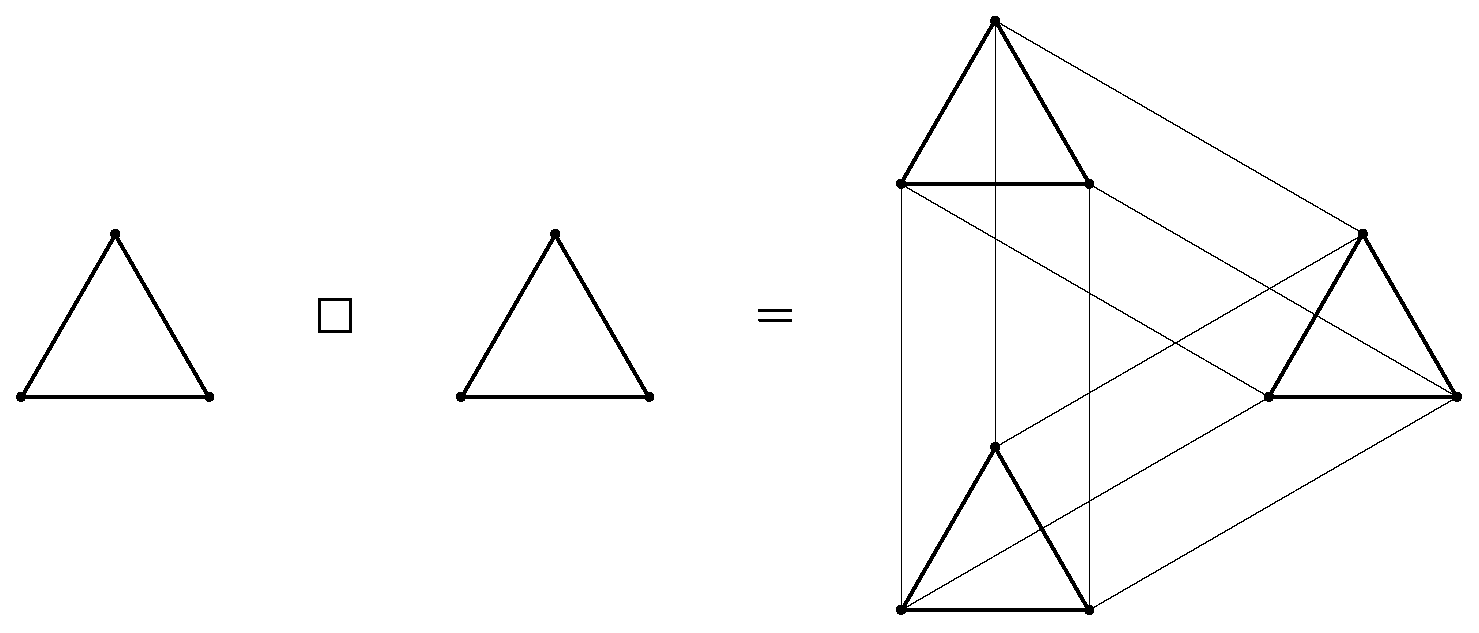
\includegraphics[width=0.5\linewidth]{Figures/GraphProd.eps}
    \caption{$\CompleteGraph_3 \square \Cycle_3$}
    \label{fig:GraphProd}
\end{figure}

The Cartesian product preserves several important structural properties of graphs, as established in the classical work of Sabidussi. In particular, regularity and chromatic number behave additively and maximally, respectively, under graph products.

\begin{proposition}[Lemma 2.5--2.6 in~\cite{Sabidussi_1957}]
\label{prop:SabidussiCombinedGeneral}
Let $\GraphG$ and $\GraphH$ be graphs. Then:
\begin{enumerate}
    \item If $\GraphG$ is $r$-regular and $\GraphH$ is $s$-regular, then the Cartesian product $\GraphG \square \GraphH$ is $(r+s)$-regular. \label{GraphProdReg}
    \item The chromatic number of the Cartesian product satisfies
    \[
    \chi(\GraphG \square \GraphH) \;=\; \max\{\chi(\GraphG),\, \chi(\GraphH)\}. \label{GraphProdChrom}
    \]
\end{enumerate}
\end{proposition}

The second item in Proposition~\ref{prop:SabidussiCombinedGeneral} immediately yields an upper bound on clique number, since for every graph $\GraphG$ it is well known that $\omega(\GraphG) \leq \chi(\GraphG)$. Of special relevance to our construction are Cartesian products in which one factor is a cycle graph $\Cycle_\enn$. A particularly notable subclass is obtained when the other factor is a complete graph $\CompleteGraph_\arr$: the graphs $\CompleteGraph_\arr \square \Cycle_\enn$ are referred to as \emph{KC-graphs}, a terminology introduced by Knuth~\cite{Knuth:TAOCP4F7} and further discussed in the combinatorial literature~\cite{Knuth:CoupsGracefulGraphs,MathWorld:KCGraph}.

The following observation records the immediate consequences of these observations for clique structure in graph products.

\begin{observation}\label{obs:ProdCliqInvs}
    Let $\GraphG$ and $\GraphH$ be arbitrary graphs, let $\CompleteGraph_\arr$ denote the complete graph on $\arr$ vertices, and let $\Cycle_\enn$ denote the $\enn$-cycle. Then:
    \begin{enumerate}
        \item $\omega(\GraphG \square \GraphH) \leq \max\{\chi(\GraphG),\, \chi(\GraphH)\}$. \label{ProdCliqInvsGH}
        \item $\omega(\GraphG \square \Cycle_\enn) = \omega(\GraphG)$ for all $\omega(\GraphG) \geq 3$. \label{ProdCliqInvsGC}
        \item $\omega(\CompleteGraph_\arr \square \Cycle_\enn) = \arr$ for all $\arr \geq 3$ \label{ProdCliqInvsKC}
    \end{enumerate}
\end{observation}


% The Cartesian product preserves many structural properties of graphs. 

% \begin{proposition}[Lemma 2.5-2.6 in~\cite{Sabidussi_1957}]
% \label{prop:SabidussiCombinedGeneral}
% Let $\GraphG$ and $\GraphH$ be graphs. Then:
% \begin{enumerate}
%     \item If $\GraphG$ is $r$-regular and $\GraphH$ is $s$-regular, then the Cartesian product $\GraphG \square \GraphH$ is $(r+s)$-regular. \label{GraphProdReg}
%     \item The chromatic number of the Cartesian product satisfies
%     $\chi(\GraphG \square \GraphH) \;=\; \max\{\chi(\GraphG),\, \chi(\GraphH)\}.$ \label{GraphProdChrom}
% \end{enumerate}
% \end{proposition}

% Point \ref{GraphProdChrom} of the Proposition \ref{prop:SabidussiCombinedGeneral} also serves as an upper bound on the clique number of a graph since it is well known that the for any graph $\GraphG$, $\omega(\GraphG) \leq \chi(\GraphG)$. Of particular interest in this work will be the class of graph products, when one of the factors is a cycle graph $\Cycle_\enn$. An interesting subclass of these graphs are those graphs consisting of the cartesian product of a complete graph $\CompleteGraph_\arr$ and $\Cycle_\enn$. Such graphs are known as \emph{KC-graphs} \cite{MathWorld:KCGraph} as coined by donald knuth in \cite{Knuth:TAOCP4F7}. We summarize the above observations in the following proposition.

% \begin{proposition}\label{prop:ProdCliqInvs}
%     Let $\GraphG$ and $\GraphH$ be arbitrary graphs, let $\CompleteGraph_\arr$ be the complete graph on $\arr$ vertices and let $\Cycle_\enn$ be the $\enn$-cycle. Then,

%     \begin{enumerate}
%         \item $\omega(\GraphG \square \GraphH) \leq \max\{\chi(\GraphG),\, \chi(\GraphH)\}$
%         \item $\omega(\GraphG \square \Cycle_\enn) = \omega(\GraphG)$, for $\omega(\GraphG) \geq 3$
%     \end{enumerate}
% \end{proposition}



% \begin{proposition}[Lemma 2.5 \cite{Sabidussi_1957}]\label{prop:GraphProdReg}
%     Let $\GraphG$ be an $r$-regular graph. Then $\GraphG \square C_2$ is $(r+1)$-regular and $\GraphG \square C_\enn$ is $(r+2)$-regular for any $n \geq 3$.
% \end{proposition}

% \begin{proposition}[Lemma 2.6 \cite{Sabidussi_1957}]\label{prop:ProdChromInvs}
%     For any graph $\GraphG$ and cycle $\Cycle_\enn$ on $n \in \N$ vertices, $\chi(\GraphG) = \chi(\GraphG \square C_\enn)$. 
% \end{proposition}



% \begin{lemma}\label{lem:clique-number-Gks}
% For every integer $\kay \ge 3$ and every $\ess \in \N$, the clique number of
% $\GraphG_\ess^\kay$ satisfies
% \[
% \omega(\GraphG_\ess^\kay) = \kay.
% \]
% \end{lemma}
% \begin{proof}
% Recall that by definition
% \[
% \GraphG_\ess^\kay = (K_\kay \square C_2) \square C_{\ess+1},
% \]
% and the Cartesian product is associative up to isomorphism. For $\ess = 0$,
% we also allow the interpretation $C_1$ as the trivial graph on a single
% vertex, in which case $\GraphG_0^\kay \cong K_\kay \square C_2$.

% We first record a general observation about Cartesian products with a complete
% graph.

% \medskip
% \noindent\emph{Claim.}
% Let $\kay \ge 1$ and let $H$ be any graph. Then
% \[
% \omega(K_\kay \square H) = \max\{\kay,\omega(H)\}.
% \]

% \noindent\emph{Proof of the claim.}
% Clearly $K_\kay \square H$ contains an induced copy of $K_\kay$ for each
% vertex of $H$ (fix the second coordinate), and an induced copy of $H$ for
% each vertex of $K_\kay$ (fix the first coordinate). Thus
% $\omega(K_\kay \square H) \ge \max\{\kay,\omega(H)\}$.

% For the reverse inequality, let $C$ be a clique in $K_\kay \square H$ and
% pick any vertex $(u_0,h_0) \in C$. Every vertex $(u,h) \in C$ must be
% adjacent to $(u_0,h_0)$, and by the definition of the Cartesian product this
% is possible only if either
% \[
% u = u_0 \quad\text{and}\quad (h,h_0) \in E(H),
% \]
% or
% \[
% h = h_0 \quad\text{and}\quad (u,u_0) \in E(K_\kay).
% \]
% Hence every vertex of $C$ other than $(u_0,h_0)$ has either the same
% $K_\kay$-coordinate or the same $H$-coordinate as $(u_0,h_0)$. In
% particular, there are no vertices of $C$ with both $u \neq u_0$ and
% $h \neq h_0$.

% Partition $C \setminus \{(u_0,h_0)\}$ into
% \[
% R \eqdef \{(u,h_0) \in C : u \neq u_0\}, \qquad
% S \eqdef \{(u_0,h) \in C : h \neq h_0\}.
% \]
% If $(u,h_0) \in R$ and $(u_0,h) \in S$, then $u \neq u_0$ and $h \neq h_0$,
% so $(u,h_0)$ and $(u_0,h)$ are not adjacent in $K_\kay \square H$. Thus $C$
% cannot contain vertices of both $R$ and $S$; that is, either $R = \emptyset$
% or $S = \emptyset$.

% If $S = \emptyset$, then $C \subseteq \{(u,h_0) : u \in V(K_\kay)\}$ and
% $C$ induces a clique in $K_\kay$, so $|C| \le \kay$. If $R = \emptyset$,
% then $C \subseteq \{(u_0,h) : h \in V(H)\}$ and $C$ induces a clique in $H$,
% so $|C| \le \omega(H)$. In either case we obtain
% $|C| \le \max\{\kay,\omega(H)\}$, proving the claim.
% \hfill$\triangle$
% \medskip

% We now apply the claim to our specific graphs. By associativity of the
% Cartesian product we can rewrite
% \[
% \GraphG_\ess^\kay
% \;\cong\;
% K_\kay \square \Bigl(C_2 \square C_{\ess+1}\Bigr).
% \]
% Let us denote $H_\ess \eqdef C_2 \square C_{\ess+1}$. Since both $C_2$ and
% $C_{\ess+1}$ have clique number at most $3$, and their Cartesian product
% contains no $K_4$ (it is a grid-like graph of maximum clique size $2$ when
% $\ess+1 \neq 3$, and the triangular prism when $\ess+1 = 3$), we have
% \[
% \omega(H_\ess) \le 3.
% \]
% In particular, for all $\kay \ge 3$ and all $\ess \in \N$,
% \[
% \omega(H_\ess) \le 3 \le \kay.
% \]

% Applying the claim with $H = H_\ess$ now gives
% \[
% \omega(\GraphG_\ess^\kay)
% = \omega\bigl(K_\kay \square H_\ess\bigr)
% = \max\{\kay,\omega(H_\ess)\}
% = \kay,
% \]
% as desired.
% \end{proof}



\subsection{Vertex Classification and the Weisfeiler--Leman Refinement}

A fundamental tool for reasoning about graph structure is the \emph{Weisfeiler--Leman (WL) algorithm}, also called \emph{color refinement} or \emph{vertex classification}. Originally introduced by Weisfeiler and Leman~\cite{Weisfeiler:1968ve}, the WL method is an iterative vertex-coloring procedure designed to detect whether two graphs are non-isomorphic.

Given a (possibly vertex-labeled) graph $G = (V,E)$ and an initial labeling $\lambda^{(0)} : V \to \Sigma$, the 1-WL algorithm constructs a sequence of colorings $\lambda^{(t)} : V \to \Sigma$ where each $\lambda^{(t)}$ refines the structural information of $\lambda^{(t-1)}$. For each integer $t \ge 1$ and each vertex $v \in V$, we define
\[
\lambda^{(t)}(v)
    = \mathrm{HASH}\!\left(
        \lambda^{(t-1)}(v),~
        \big\{\!\!\{\lambda^{(t-1)}(u) : u \in N(v)\}\!\!\}
    \right),
\]
where $N(v)$ is the neighborhood of $v$ and $\mathrm{HASH}$ bijectively maps each pair consisting of a color and a multiset of colors to a fresh symbol not used previously. Intuitively, each vertex updates its color using its own prior color together with the multiset of colors of its neighbors.

Running the WL refinement simultaneously on two graphs $G$ and $H$, the algorithm concludes that the graphs are \emph{not isomorphic} if, at any refinement step $t$, the two colorings assign different numbers of vertices to some color class. 
If no such discrepancy is detected, the algorithm continues until stabilization, which occurs at the first iteration $t$ for which the number of colors remains unchanged, i.e., when the colorings at iterations $t-1$ and $t$ have images of equal cardinality. As the number of colors is bounded by the number of vertices, termination is guaranteed within $\max\{|V(G)|,|V(H)|\}$ iterations.
. The resulting stable coloring of $G$ will be denoted $\WL(G)$ and is also called the \emph{vertex-classification type} of $G$.

Despite its effectiveness on most graph instances, the 1-WL refinement has well-understood
limitations. In particular, it completely fails to extract structural information from regular
graphs: when every vertex has the same degree, all neighborhoods appear identical at every
refinement round \cite{WeisfeilerLehmanMethod,LowerBoundGraphIdentification}. As a consequence, 1-WL assigns the same color to all vertices in any
regular graph, and therefore cannot distinguish between non-isomorphic regular graphs that
share the same number of vertices. We formalize this in the following observation in order to refer to it later.


\begin{observation}
\label{obs:WL-regular-undistinguished}
Let $G$ and $H$ be $r$-regular graphs on the same number of vertices.
Then $1$-WL produces only a single color class on both $G$ and $H$.
In particular, $\WL(G) \cong \WL(H)$.
\end{observation}


% \begin{proof}
% Initially, every vertex in $G$ has the same color by assumption. Since $G$ is $r$-regular, every vertex has exactly $r$ neighbors and hence the multiset of neighbor colors is identical for all vertices. Thus the update rule of $1$-WL assigns the same new color to every vertex in the next iteration. The same argument applies inductively for all subsequent rounds, showing that $\lambda^{(t)}$ remains constant for all $t \ge 0$. The claim for $H$ follows analogously. Therefore the stable colorings of $G$ and $H$ each contain a single color class, and hence $1$-WL cannot distinguish the two graphs.
% \end{proof}


% The expressive power of the WL refinement is closely tied to modern graph neural networks (GNNs) based on message-passing. The following result has become standard in the GNN literature.


% \begin{proposition}[Find citation!!]\label{prop:VertClass}
%     Let $\GraphG$ and $\GraphH$ be graphs where $|\VertexSet(G)| = |\VertexSet(G)|$. If $\reg(\GraphG) = \reg(\GraphH)$, then $\VertClass(\GraphG) = \VertClass(\GraphH)$.
% \end{proposition}

\subsection{Graph Neural Networks}
\label{subsec:GNNs}

Graph neural networks (GNNs) are neural architectures designed to operate on graphs.
Given a graph $G = (V,E)$ with (optional) node feature vectors $\mathbf{x}_v$ for each
$v \in V$, a GNN computes hidden representations for nodes by iteratively aggregating
information from local neighborhoods. This paradigm is commonly referred to as
\emph{message passing} or \emph{neighborhood aggregation}
\cite{HamiltonYingLeskovec2017b, KipfWelling2017, GilmerEtAl2017}.

A generic layer of a message-passing GNN updates each node representation as follows:
\[
\mathbf{h}_v^{(t)} = 
\mathrm{UPDATE}^{(t)} \!\left(
    \mathbf{h}_v^{(t-1)},
    \mathrm{AGG}^{(t)}\bigl\{ \mathbf{h}_u^{(t-1)} : u \in N(v) \bigr\}
\right),
\]
where $\mathbf{h}_v^{(0)} := \mathbf{x}_v$ initializes the process,
and both $\mathrm{UPDATE}^{(t)}$ and $\mathrm{AGG}^{(t)}$ are learnable,
permutation-invariant functions (e.g.\ neural networks).
After $T$ iterations, node representations incorporate structural information up to
their $T$-hop neighborhoods.

For graph-level prediction tasks (such as graph classification),
a final \emph{readout} operator aggregates the node representations:
\[
\mathbf{h}_G 
    = \mathrm{READOUT}\bigl(\{\mathbf{h}_v^{(T)} : v \in V\}\bigr),
\]
where $\mathrm{READOUT}$ is also permutation invariant (typically sum, mean, or max).

GNNs have achieved strong empirical success across numerous domains including
computational chemistry, physics, social network analysis, and algorithmic reasoning
tasks~\cite{BronsteinEtAl2021, BattagliaEtAl2018}.
Their defining characteristic is that all computations respect the
graph’s combinatorial symmetries: permuting vertex labels does not change the output.

A fundamental expressive limitation of GNNs, explored in prior work
\cite{XuEtAl2019, MorrisEtAl2019}, is that message-passing architectures are at most as powerful as
the 1-dimensional Weisfeiler--Leman refinement (Section~\ref{subsec:WL}):
they cannot distinguish non-isomorphic graphs that receive the same stable coloring under 1-WL.
This connection will play a central role in our hardness construction.

\begin{proposition}[Thm. 1 in ~\cite{MorrisEtAl2019}, Lemma 2 in \cite{XuEtAl2019}]
\label{prop:WLvsGNN}
Let $\GNN$ be any message-passing graph neural network. If $\WL(G) \cong \WL(H)$, then
$\GNN(G) = \GNN(H)$.


\end{proposition}

In other words, GNNs cannot distinguish graphs that are indistinguishable by the 1-WL algorithm.
Thus, the 1-WL refinement characterizes the \emph{exact} expressive limitations of message-passing GNNs: any pair of graphs that the WL refinement fails to separate cannot be separated by such neural architectures, regardless of architecture or training.

While Proposition~\ref{prop:WLvsGNN} establishes that GNNs cannot exceed the expressive
capabilities of the 1-WL refinement, it is equally important that this limitation is tight.
In fact, prior work has shown that message-passing GNNs can simulate the behavior of 1-WL
exactly, provided that the aggregation and update functions are sufficiently expressive and
injective~\cite{XuEtAl2019, MorrisEtAl2019}. Thus, the expressive power of GNNs is
\emph{precisely} characterized by the Weisfeiler--Leman algorithm.

\begin{proposition}[Thm. 3 in \cite{XuEtAl2019}, Thm. 2 in \cite{MorrisEtAl2019}] \todo{Check that the statment of this Prop is sound according to the cited papers. It should be, "There exist aggregation functions such that..."}
\label{prop:GNN-iff-WL}
Let $\mathcal{N}$ be a message-passing graph neural network whose aggregation and update
functions are injective. Then for any two graphs $G$ and $H$ and any $t \ge 0$,
\[
\WL(G) \cong \WL(H)
\quad\Longleftrightarrow\quad
\mathcal{N}(G) = \mathcal{N}(H).
\]
\end{proposition}
In particular, $\mathcal{N}$ distinguishes exactly the same pairs of graphs as the 1-dimensional WL test.
\noindent
Therefore, to prove that certain graph pairs are hard for all message-passing GNNs, it suffices
to exhibit pairs that are indistinguishable by 1-WL. This observation forms the basis for the
hard graph families constructed in section \ref{sec:HardFamilies}.


\subsection{$k$-Dimensional Weisfeiler--Leman and $k$-GNNs}

The Weisfeiler--Leman (WL) refinement admits a natural higher-dimensional generalization known as the $k$-dimensional WL procedure ($k$-WL). For a graph $\GraphG$ with vertex set $V(\GraphG)$ and a fixed integer $k \ge 2$, the $k$-WL algorithm operates on ordered or unordered $k$-tuples of vertices. In this work, we follow the \emph{set-based} formulation used in~\cite{MorrisEtAl2019}, which considers the collection $[V(\GraphG)]^k$ of all $k$-element subsets of $V(\GraphG)$.

For a $k$-set $s = \{s_1,\dots,s_k\} \in [V(\GraphG)]^k$, the neighborhood of $s$ is defined as
\[
N(s) \;=\; \{\, t \in [V(\GraphG)]^k \mid |s \cap t| = k-1 \,\}.
\]
That is, two $k$-sets are neighbors if they differ in exactly one vertex.

The set-based $k$-WL refinement proceeds analogously to the classical $1$-WL algorithm. It computes a sequence of colorings
\[
c^{(t)}_{s,k,l} : [V(\GraphG)]^k \rightarrow \Sigma,
\]
where the initial coloring $c^{(0)}_{s,k,l}$ assigns to each $k$-set $s$ the isomorphism type of the induced subgraph $\GraphG[s]$ (taking vertex labels into account, if present). In each subsequent iteration, the color of $s$ is updated based on its previous color together with the multiset of colors of its neighbors. As in the $1$-dimensional case, the refinement stabilizes once no further color refinement is possible.

Motivated by this higher-dimensional refinement, Morris et al.~\cite{MorrisEtAl2019} introduced \emph{$k$-dimensional graph neural networks} ($k$-GNNs), which generalize message-passing GNNs by lifting computation from vertices to $k$-sets. Given a labeled graph $(\GraphG,l)$, a $k$-GNN associates to each $k$-set $s \in [V(\GraphG)]^k$ a feature vector $f_k^{(t)}(s)$ at layer $t \ge 0$. The initial features $f_k^{(0)}(s)$ are chosen as a one-hot encoding of the isomorphism type of $\GraphG[s]$.

For $t > 0$, features are updated according to the rule
\[
f_k^{(t)}(s)
\;=\;
\sigma\!\left(
f_k^{(t-1)}(s)\, W_1^{(t)}
\;+\;
\sum_{u \in N(s) } f_k^{(t-1)}(u)\, W_2^{(t)}
\right)
\]
where $W_1^{(t)}, W_2^{(t)}$ are learnable weight matrices and $\sigma$ is a non-linear activation function. 

A key theoretical result established in~\cite{MorrisEtAl2019} is that $k$-GNNs are tightly connected to the $k$-WL refinement. In particular, for any labeled graph $(\GraphG,l)$ and any $k \ge 2$, the features computed by a $k$-GNN are bounded in expressive power by the corresponding $k$-WL coloring, and conversely, there exist choices of weights such that $k$-GNNs exactly simulate the set-based $k$-WL refinement at every iteration.

Consequently, the distinguishing power of $k$-GNNs coincides exactly with that of the set-based $k$-WL refinement.


\begin{proposition}[{\cite{MorrisEtAl2019}}]
\label{prop:kGNN-iff-kWL}
Let $(\GraphG,l)$ and $(\GraphH,l')$ be labeled graphs and let $k \ge 2$. Then for any $t \ge 0$ there exists some $k$-GNN $\mathcal{N}_k$ such that,
\[
c^{(t)}_{s,k,l}(\GraphG) \;\cong\; c^{(t)}_{s,k,l'}(\GraphH)
\quad\Longleftrightarrow\quad
\mathcal{N}_k^{(t)}(\GraphG) = \mathcal{N}_k^{(t)}(\GraphH),
\]
where $c^{(t)}_{s,k,l}$, denotes the set-based $k$-WL coloring after $t$ refinement steps.
\end{proposition}





% \subsection{Graph Neural Networks}

% \begin{proposition}[Find citation!!]
% \label{prop:gnn-wl}
% Let $\GNN$ be any message-passing graph neural network. If $\VertClass(\GraphG) \cong \VertClass(\GraphG')$, then $\GNN(G) = \GNN(G')$.

% \end{proposition}